\chapter{Related Work}
In this chapter we examine some of the key features which were taken into account when creating the Feed Bundle Protocol. Before taking a closer at the baseline for the protocol, which consists of parts from the Secure Scuttlebutt technology [\citenum{ssbc}] and the Remote Procedure Call Protocol, we will quickly jump into the blockchain and its properties, everybody who reads this thesis will have heard about it by now.
\section{Blockchain}
The blockchain has already proven its importance and application as the foundation of an alternative currency called the Bitcoin [\citenum{swan2015blockchain}]. It has received an extensive attention in recent years [\citenum{8029379}]. But what is it that makes the blockchain so impressive and desired? The blockchain is described by \citet{8029379} as an immutable ledger which allows transactions to take place in a decentralised manner. 
As described by \citet{swan2015blockchain}, the so called blocks are added to the blockchain in a linear, chronological order, whereas once a block is added and validated, it cannot be removed from the chain. Exactly these key properties we also find in Secure Scuttlebutt.
\section{Secure Scuttlebutt}
Having a rather well known append-only log like the blockchain as a foundation and rather well know by the broad mass makes the jump into the the universe of Secure Scuttlebutt much easier. Secure Scuttlebutt is a novel peer-to-peer event-sharing protocol and architecture for social apps [\citenum{tarr2019secure}]. The aim of this section is to give a very high level overview about SSB, its ideas and properties, since the they are not quite easy to understand.

\subsection{Append-Only Log}
Given the ID-centric architecture of Scuttlebutt, where one identity belongs to one feed, which is replicated to each of its peers, we clearly see the novelty of this approach. Instead of having central servers, which hold all the data about its users, every user has a copy of the entire database of their own network. So, information can also be gathered offline, without connecting to the old-fashioned server. 

\begin{figure}
    \centering
    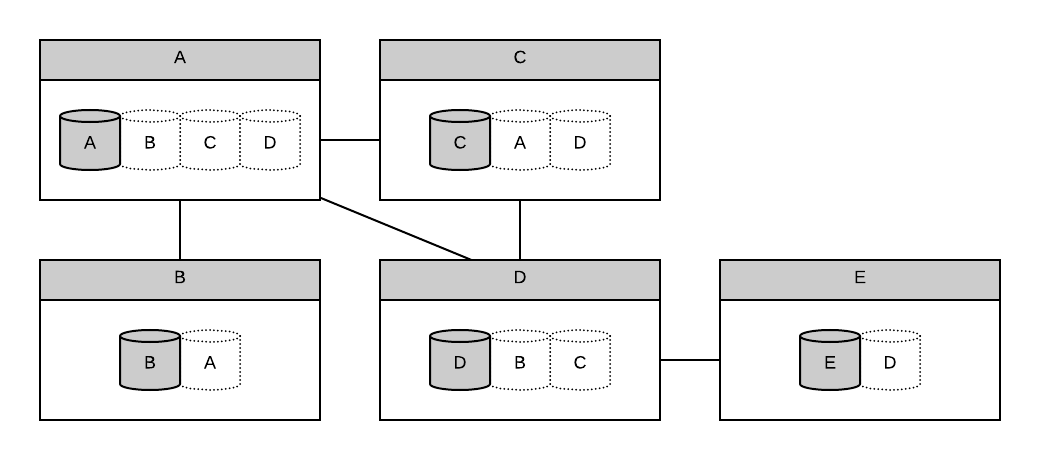
\includegraphics[width=0.8\textwidth]{ssb_raw}
    \caption{A simplified SSB network.}
    \label{fig:sbb-raw}
\end{figure}

Having this, not a company, for example Facebook, will hold your data. Instead, you and all your peers hold each others data locally in their machines. Therefore, no central instance has complete control about the data inside the network. The database is distributed all over the network in several append-only logs with information about the specific identity [\citenum{ssbc}]. Everything ever created is saved inside these logs, even unnecessary data. Over time these logs grow and have enormous space complexity, up to a point where the networks bandwith is completely exhausted from the replicaton process. One approach by \citet{entropy} to solve this is only replicating data one peer does not contain. Specifically, packets that are beyond the entropy frontier. Another is to split the feeds in several feeds and have more "channels", this approach is considered in this thesis.
This must be considered if Secure Scuttlebutt wants to establish as a reliable social network amongst its competitors.\footnote{P2P-Basel [\citenum{p2pbasel}]}

\subsection{Onboarding}
Onboarding into the Secure Scuttlebutt social media network differs from the the common way to join a social media network. First of all, the key pair is needed as well as the feed describet above [\citenum{ssbc}]. Not every application has a built in identity generation. Therefore, it cannot be downloaded every SSB-client to enter SSB.\footnote{P2P-Basel [\citenum{p2pbasel}]} On of the clients, which have a out of the box identity generation mechanism is Patchwork [\citenum{patchwork}]. If finally an identity is created, Secure Scuttlebutt has two ways for peers to discover each other [\citenum{ssbc}]. First, the constant broadcasting of UDP-packets allows identities in the same network to discover each other. In the real world this corresponds to standing in the streets and just yell and wait until someone notices you. Second, a user can connetct to a pub [\citenum{pubs}] via an invite code. This results in you following the pub and the pub instantly following you back. Now the feed of the pub can be seen as well as the feeds of its peers. These invite codes are distributed which ever way the pub operator desires. No general channel for invite codes is given. Here the real world analogy suits very well, going in a pub and meet new people, but the address of the pub must be self found. 
\\
Concluding, the first ways are based on luck, which is not very promising in the long run. They are based on luck, because the user has no idea what other people he encounters. There is no "map" which holds the location of pubs. Therefore an "all-knowing", trusted middle-man is an appropriate addtion to take account of.
\section{Remote Procedure Call}
Remote procedure calls [\citenum{birrell1984implementing}], as the name implies, are based on procedure calls but extended
to provide for transfer of control and data across a communication network. There are
two participants in the simplest manner, the caller and the callee. The caller wants to invoke a
procedure with given parameters. The callee is the instance, which actually proceeds with
the data and returns the result of that specific request. If an RPC is invoked, the the caller’s
environment is supended and all the information needed for the call transmitted is through the
network and received by the callee, where the actual procedure is executed with these exact
parameters. The benefit of such an RPC-protocol is that the interfaces are designed in a
way that third parties only write the procedures and call exactly these procedures in the
callers environment [\citenum{birrell1984implementing}] This leads to a very promising basic version of such
an RPC-protocol for this thesis, since it allows the caller to invoke the procedure in the caller's own  environment, but the procedure is actually performend by a callee, which returns the result back to the caller[\citenum{birrell1984implementing}].